\section{数据库设计}

\subsection{大数据分析模块}
大数据分析模块负责进行数据的处理,它的整体框架图是这样的:
\begin{figure}[!htbp]
	\centering
	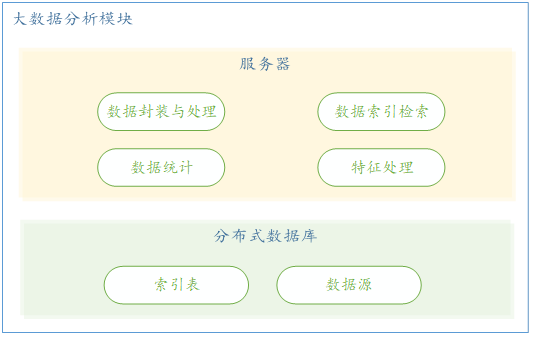
\includegraphics[scale=0.4]{image/d1.png}
	\caption{大数据分析模块}
\end{figure}

\subsection{数据存储系统的设计与实现}
\textbf{介绍}
数据存储系统是大数据可视化的基础,是整个系统的根脉。
对于存储的大量数据进行统计,计算和处理通常需要以小时和天为记的时间,而本系统的用户会根据需要对于已经处理好的数据进行可视化定制。所以数据存储系统的设计需要满足以下用户需求:
	对已处理的数据进行可视化渲染
	对结构简单的数据进行多样化的渲染,比如同时渲染成柱状图和饼图
	对渲染的低延时需求,需要“即做即画”
	对某组数据进行快速索引,通过少量关键字迅速检索需要的数据

基于以上需求特点,本系统采用Hadoop生态中的HBase存储方案,该方案具有以下特点:
	擅长存储半结构化数据,存储结构灵活
	面向列的设计使得一张表中可以存储数以万计的不同图表数据
	可以提供低延时查询,通过行键的查询延时在1ms内
HBase是基于HDFS和MapReduce的大数据存储框架,易上手、可扩展、高容错,在分布式存储方案中非常流行。本系统也使用HBase存储需要可视化的数据集。

\textbf{HBase的基本存储方式}
\begin{itemize}
\item 表名
\end{itemize}

\begin{table}[!htbp]
	\centering
	\caption{表名}
	\label{tab:my-table}
	\begin{tabular}{|l|l|l|}
		\hline
		行键 & 列族 \\ \hline
		通过键值检索行 & 在创建表时定义所有列族  \\ \hline
		通常存储全表最关键的索引信息 & 每行中每个列族可以存储任意多列 \\ \hline
		一个行键的大小最大为单元格大小 & 一行和一个列族和一个列对应一个单元格 \\ \hline
        行键在全表中唯一 & 可以重复,不同的单元格用时间戳区分 \\ \hline
        每一行的每个列族下的列都不一定一样 & 可以重复,不同的单元格用时间戳区分,查询时一般查询最新单元格 \\ \hline
	\end{tabular}
\end{table}

可以看到,HBase基于列的表结构非常适合本系统中不同图表具有不同的数据列的特点。所有经过处理的图表数据可以全部存储在一张HBase表中,通过表名进行快速检索,真正做到“即做即画”的实时数据渲染的要求。

